%!TEX root = ../Thesis.tex

\chapter{Einleitung}
\label{cha:introduction}

Staus und zäh fließender Verkehr sind sowohl auf Schnell- und Autobahnen, als auch in Städten ein großes
Problem und Ärgernis für Autofahrer. Sie kosten diese nicht nur wertvolle Zeit, sondern auch viel Geld.
Laut einer Studie von \cite[]{Cookson} kosten Staus jeden deutschen Autofahren pro Jahr durchschnittlich 1770 €.
In Summe ergeben sich hieraus beinahe 80 Milliarden Euro an Kosten.
Staus sind allerdings nicht nur finanziell für Privatpersonen oder Unternehmen ein Problem,
sondern sie erhöhen auch das Unfallrisiko und tragen maßgeblich zur schlechten Luftqualität in Innenstädten bei.
Aufgrund längerer Fahrzeiten und der häufigen Be- und Entschleunigung, steigt der Kraftstoffverbrauch der
Fahrzeuge und dadurch auch die Schadstoffbelastung in der Luft \cite[]{Hemmerle2016}.

Die wichtigste Voraussetzung, um Staus präventiv entgegenwirken zu können, ist, den Verkehr so gut wie
möglich zu verstehen. Nötig ist ein Verständnis des Straßenverkehrs als Ganzes, sowie der Auswirkungen,
welche einzelne Verkehrsteilnehmer und deren Verhalten, auf diesen haben. Hierzu ist das Erstellen von
Simulationen sowie die Auswertung realer Verkehrsaufkommen in Analysen unerlässlich.
Die auf diese Weise gesammelten Erkenntnisse bilden die Grundlage, um Straßenabschnitte und Infrastrukturanlagen
wie Ampeln, insbesondere auch in Innenstädten, intelligent zu gestalten. In Zukünft könnten auch
autonome Fahrzeuge von Erkenntnissen aus Verkehrsanalysen profitieren.

Dank der Tatsache, dass unbemannte Luftfahrzeuge (\acrshort*{uav}) wie Drohnen immer leichter und günstiger
verfügbar sind, und die von ihnen erstellten Aufnahmen teils eine sehr gute Qualität besitzen, werden
diese immer häufiger zur Analyse des Straßenverkehrs eingesetzt. Über Methoden aus dem Umfeld des
maschinellen Sehens und maschinellen Lernens können aus Luftaufnahmen eine Vielzahl an interessanter
Informationen extrahiert werden.

Diese Arbeit beschäftigt sich mit der Realisierung einer automatischen Fahrspurerkennung in Luftaufnahmen.
Hierzu werden die Trajektoriedaten von Fahrzeugen ausgewertet, welche aus Luftaufnahmen rekonstruiert wurden.
Die Analyse von Verkehrssituationen wird, aufgrund der oben genannten Probleme und der zunehmenden Relevanz
des autonomen Fahrens, immer wichtiger.
Eine automatisierte Spurerkennung ist ein wichtiger Teil des Analyseprozesses, da mit Hilfe der
erkannten Spuren unter anderem Spurwechsel- und Überholvorgänge sowie das Verhalten der Fahrzeuge
auf einer Spur untereinander untersucht werden können.

\section{Rahmen der Arbeit}
\label{sec:rahmen_arbeit}

Diese Masterthesis wurde im Rahmen des Forschungsprojektes MEC-View umgesetzt. Das Projekt und dessen
Teilprojekt Luftbeobachtung wird nachfolgend vorgestellt.

\subsection{Das Projekt MEC-View}
\label{sec:mec_view}

Das Forschungsprojekt MEC-View, welches vom Bundesministerium für Wirtschaft und Energie (BMWi) gefordert wird,
hat das Ziel, autonomes Fahren im urbanen Raum zu ermöglichen und für alle Verkehrsteilnehmer sicher zu gestalten.
Gerade in Innenstädten sind die Möglichkeiten des autonomen Fahrens, aufgrund von unübersichtlichen Kreuzungen,
Fußgängern und Fahrradfahrern, verdeckten Sichten und anderen Faktoren, begrenzt.
Abbildung \ref{fig:intro_mec_view_arch} gibt einen Überblick über das Forschungsprojekt und veranschaulicht dessen Ziel.

\begin{figure}[H]
\centering
    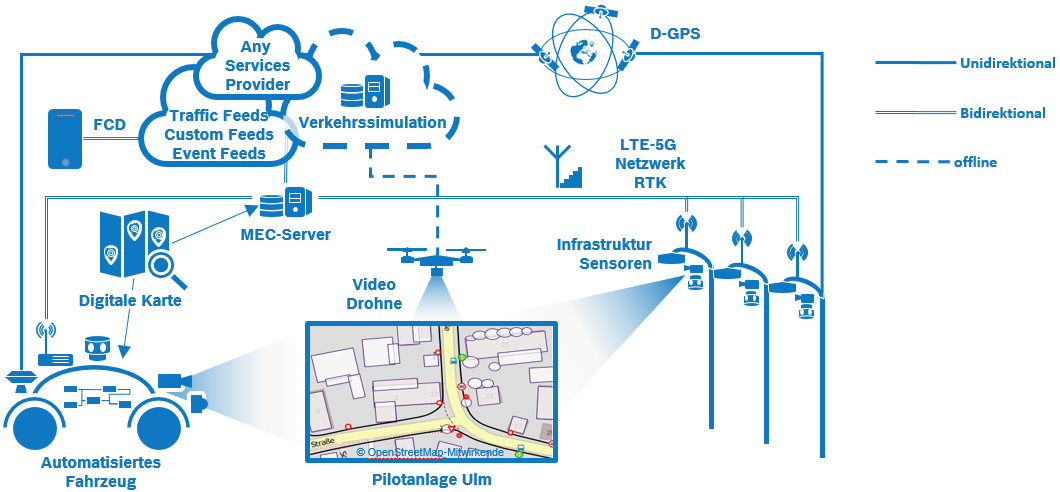
\includegraphics[width=0.7\linewidth]{resources/img/mec_view_arch}
\caption[Überblick MEC-View Projekt]{Überblick MEC-View Projekt \cite[]{mecViewWeb}}
\label{fig:intro_mec_view_arch}
\end{figure}

In urbanen Gebieten
sollen neben Daten von fahrzeuginternen Sensoren auch Informationen externer Infrastruktur-Sensoren verwendet werden,
damit autonome Fahrzeuge eine fundierte Verhaltensentscheidung auf Basis eines detaillierten Umfeldmodells treffen können.
Im Rahmen des Forschungsprojektes MEC-View wird eine Pilot-Anlage zur Umfelderfassung an einer vorfahrtberechtigten Straßenkreuzung
in Ulm aufgebaut und getestet. In dieser Anlage werden die Verkehrsteilnehmer über Kameras und LIDAR-Sensoren erfasst
und die ermittelten Daten über ein schnelles LTE/5G-Mobilfunknetz an einen \textit{Mobile Edge Computing} (\acrshort*{mec}) Server übertragen.
Hier werden die Daten in Echtzeit zu einem Umfeldmodell fusioniert, welches anschließend den autonomen Fahrzeugen
zur besseren Navigation zur Verfügung gestellt wird. Beteiligt an diesem Forschungsprojekt sind neben
der IT-Designers GmbH unter anderem auch die Daimler AG, die Robert Bosch GmbH, Osram, Nokia und die Universität Ulm.
Jeder Projektpartner ist verantwortlich für unterschiedliche Teilaspekte des Projektes. Die IT-Designers GmbH,
bei welcher diese Arbeit angefertigt wird, entwickelt den MEC-Server und ist verantwortlich für das
Teilprojekt \textit{Luftbeobachtung}. \cite[]{mecViewWeb}

\subsection{Das MEC-View Teilprojekt Luftbeobachtung}
\label{sec:mecview_sim}

Im MEC-View Teilprojekt \textit{Luftbeobachtung} werden Verkehrsanalysen und Simulationen erstellt, welche dabei helfen
das Verhalten des Verkehrs besser zu verstehen und es somit ermöglichen, diesen zu optimieren.
Mithilfe der Analysen kann beispielsweise untersucht werden, wie durch die Anpassung von Verkehrssteuerungsanlagen
oder durch die Änderung des Fahrverhaltens einzelner Fahrzeuge, eine Verbesserung der Verkehrssituation erreicht werden kann.
Die Erkenntnisse können insbesondere auch in die Verhaltenssteuerung von autonomen Fahrzeugen mit einfließen.
Aus diesem Grund sind entsprechende Untersuchungen auch für das MEC-View Hauptprojekt relevant.

Die Untersuchungen werden im MEC-View Projekt anhand von Luftbeobachtungen durchgeführt, welche von Drohnen getätigt werden.
In den Videoaufnahmen werden mithilfe eines neuronalen Netzes die Positionen und Fahrzeugklassen der Verkehrsteilnehmer ermittelt.
Mittels dieser kann anschließend beispielsweise die Geschwindigkeit und Beschleunigung der einzelnen Fahrzeuge bestimmt werden.
Zur Erstellung der Analysen ist es zudem wichtig, eine Kenntnis der Topologie der untersuchten Straßen, das heißt des
Verlaufs der Fahrbahnen und Spuren, zu besitzen. In Kombination mit den Fahrzeugpositionen können so interessante
Kenngrößen wie der Verkehrsfluss oder die Verkehrsdichte ermittelt werden.

\section{Motivation und Ziele}
\label{sec:motivation_goals}

Im Rahmen dieser Arbeit wird ein Verfahren zur automatischen Erkennung von Fahrspuren in Luftaufnahmen
auf Basis von Trajektoriedaten entwickelt. Die Spurerkennung wird in die Anwendung \textit{Vehicle-Tracker}
integriert, welche im Rahmen des MEC-View Luftbeobachtungs Projekt erstellt wird. Sie dient der Auswertung
von Luftbeobachtungen des Straßenverkehrs.
In der \textit{Vehicle-Tracker} Applikation mussten bislang die Fahrspurverläufe in jeder Aufnahme
händisch definiert werden. Dieser Prozess ist insbesondere dann aufwendig, wenn die zu untersuchenden
Straßenabschnitte beispielsweise mehrspurige Kreuzungen oder Kreisverkehre beinhalten. Das in dieser Arbeit
entwickelte Spurerkennungs-Modul soll die manuelle Spur-Definition weitestgehend ersetzen und es so ermöglichen
in Zukunft mehr Luftaufnahmen mit weniger Aufwand auszuwerten.

Der Verlauf und die Geometrie der Fahrspuren wird in dieser Thesis anhand der Bewegungsbahnen von Fahrzeugen, den sogenannten Trajektorien,
ermittelt. Im Gegensatz zu einer visuellen Detektierung hat das Verfahren den Vorteil, dass Fahrspuren auch in Aufnahmen
mit schlechten Lichtverhältnissen oder Verdeckungen der Fahrbahnen und Spurmarkierungen erkannt werden können.

Zum Thema Spurerkennung existieren zwar bereits Veröffentlichungen (siehe Abschnitt \ref{sec:rw_lane_detection}),
allerdings können die
vorgestellten Methoden meist nur in sehr speziellen Szenarien eingesetzt werden oder die erkannten Spuren
entsprechen den realen Fahrspurverläufen nur schlecht. Ziel dieser Arbeit ist es, ein Verfahren zu entwickeln,
welches Fahrspuren in möglichst vielen unterschiedlichen Szenarien erkennen kann.
Die Spuren sollen außerdem den realen Fahrbahnverläufen so gut wie möglich entsprechen.

\section{Aufbau dieser Arbeit}
\label{sec:aufbau}

Die vorliegende Arbeit ist wie folgt strukturiert:

\begin{itemize}
    \item Die zum Verständnis der Arbeit und des entwickelten Spurerkennungsalgorithmus benötigten
            Grundlagen sind in \textbf{Kapitel \ref{sec:position_extraction} und \ref{sec:tra_clustering}} beschrieben.
            Kapitel \ref{sec:position_extraction} erläutert, wie aus Luftaufnahmen die Trajektorien von Fahrzeugen
            rekonstruiert und in ein Weltkoodinatensystem überführt werden können.
            Kapitel \ref{sec:tra_clustering} stellt die grundlegenden Konzepte der Clusteranalyse vor, welche
            bei der Umsetzung der Spurerkennung zum Einsatz kommt.
    \item In \textbf{Kapitel \ref{cha:related_work}} werden verwandte Arbeiten, welche sich bereits mit
            der Thematik der Spurerkennung und der Clusteranalyse von Trajektorien befassen, vorgestellt und untersucht.
            Zudem werden Defizite der vorhandenen Lösungen und benötigte Neuerungen aufgezeigt.
    \item In \textbf{Kapitel \ref{cha:konzeption}} wird das Konzept für die Umsetzung der Spurerkennung vorgestellt.
            Es werden Anforderungen definiert und das Spurerkennungs-Modul wird in den Gesamtkontext
            der Applikation \textit{Vehicle-Tracker} eingeordnet.
    \item Nach der Konzeption wird in \textbf{Kapitel \ref{cha:realisation}} erläutert, wie die Spurerkennung konkret
            umgesetzt wurde. Es werden die verschiedenen Schritte des entwickelten Algorithmus beschrieben.
    \item In \textbf{Kapitel \ref{cha:results}} wird der entwickelte Spurerkennungsalgorithmus evaluiert.
            Es wird auf die Stärken und Schwächen der wichtigsten Verarbeitungsschritte des Algorithmus eingegangen.
            Außerdem werden die konkreten Ergebnisse in Form von Screenshots vorgestellt.
    \item \textbf{Kapitel \ref{cha:end}} bildet den Schluss dieser Masterarbeit. Hier wird
            ein Fazit gezogen und ein Ausblick gegeben, welche Verbesserungen in Zukunft an dem entwickelten
            Algorithmus noch vorgenommen werden können.
    \item Im \textbf{\hyperref[cha:anhang_a]{Anhang}} dieser Arbeit sind Aufnahmen der Straßenabschnitte dargestellt,
            mit deren Hilfe der Spurerkennungsalgorithmus entwickelt und evaluiert wurde.
\end{itemize}

